%        File: hthk6_Lik_V3.tex
%     Created: Wed Apr 25 07:00 PM 2012 G
% Last Change: Wed Apr 25 07:00 PM 2012 G
%
\documentclass[11pt,a4paper]{article}
\usepackage[icelandic]{babel}
\usepackage[T1]{fontenc}
\usepackage[utf8]{inputenc}
\usepackage{enumerate}
\usepackage{amsmath}
\usepackage{amsfonts}
\usepackage{fullpage}
\usepackage{graphicx}
\usepackage{verbatim}
\author{Nemi: Heimir Þór Kjartansson\\Verkefnakennari: Jakob Sigurðsson}
\title{Fag: Líkindaaðferðir verklegt \\ Skiladæmi 3}
\begin{document}
\maketitle
\section{Inngangur}
Hér er skoðað LTI kerfi og hegðun þess við slembið inntak. Við umfjöllun
og úrvinnslu er mikið stuðst við aðferðir og niðurstöður úr kennslubók
áfangans. Verkefnið er unnið sem þriðja verklega verkefni fyrir áfangann
Líkindaaðferðir við Háskóla Íslands.
\section{LTI kerfi}
Unnið er með LTI kerfi þar sem inntak er sett í gegnum Butterworth síu
og titlum við yfirfærslufall hennar $H(f)$. 
Aflyfirfærslufall kerfisins hefur eiginleikana
\begin{eqnarray*}
    |H(f)|^2 = \frac{1}{1+\left[\frac{f^2-f_uf_l}{f(f_u-f_l)}\right]^2}
\end{eqnarray*}
þar sem mörk síunnar eru $f_u=110Hz$ og $f_l=90Hz$.
\section{Inn- og úttak kerfisins} 
Inntakið sem skoðað er, $X(t)$, er vítt staðnað slembiferli. Skoðað 
verður úttak kerfisins, $Y(t)$.

Gefið er sjálffylgnifall innmerkisins
\begin{eqnarray*}
    R_X(\tau)=5^{-600|\tau|}
\end{eqnarray*}

Til að finna sýni úr ferli $X(t)$ er stuðst við aðferð úr námsbók úr kafla 8-11. Hvítt suð er leitt í gegnum síu
gefna með jöfnu (8-89), sjá kafla fyrir frekari útleiðslu.

Tíðnirófþéttleiki úttaksins er fundinn og settur fram sem jafna
(8-83) í námsbók og má sjá frekari atriði útleiðslu þar.
\begin{eqnarray*}
    S_Y(f)=\frac{6.0792\cdot 10^4 f^2}{f^6 -1.02811\cdot 10^4 f^4
    -7.88969\cdot 10^7 f^2 +8.93744 \cdot 10^{11}}
\end{eqnarray*}

Sýni úr inntaki og úttaki má finna með lítilvæglegri umritun á M-skrá úr 
námsbók, þ.e. ,sysxmp5.m'. Sjá hluta \ref{se:kodi} fyrir kóða. Mynd \ref{fig:X} sýnir sýni úr inntaksmerki 
og mynd \ref{fig:Y} sýnir sýni úr úttaksmerkinu.
\section{Föll sem finna rófsþéttleika} \label{se:foll}
Í hluta \ref{se:kodi} eru tilgreind þrjú föll sem hvert finnur 
rófsþéttleika. 
\begin{verbatim}
[Shat] = spect_est_pg(x, dt)
\end{verbatim}
tekur inn sýniferli $x$ og söfnunarbil $dt$ og skilar rófþéttleika 
sýniferlisins $Shat$.

Fallið fourier varpar innmerki, finnur annað veldi lengdar vörpunarinnar og deilir með lengd
innmerkisins og fæst þá rófþéttleiki. Þessi aðferð vísar mikið til skilgreiningar (7-10) úr námsbók.

\begin{verbatim}
[Shat] = spect_ext_ac(x, dt, M)
\end{verbatim}
tekur inn sýniferli $x$, söfnunarbil $dt$ og tímaseinkun $M$ og skilar
rófþéttleika sýniferlisins $Shat$.

Fallið finnur sjálffylgnifall og varpar því yfir í rófþéttleika sem við vitum að gengur skv. jöfnu (7-40) úr námsbók.
Síðar mun fallið prófað með tímaseinkun $M=16$ valið í samræmi við notkun m-skránnar ,corspec.m' í námsbók á bls. 298, 
en þetta fall er mikið byggt úr þeirri skrá.

\begin{verbatim}
[Shat] = spect_est_x(x, dt, wtype, stype)
\end{verbatim}
tekur inn sýniferli $x$, söfnunarbil $dt$, gluggategund $wtype$ þar 
sem 1 er boxcar, 2 er hamming og 3 hanning, og að lokum $stype$ 
eða róftýpu þar sem 1 er nákvæmni í tind og 2 er mýkt fall. Þá skilar
fallið rófþéttleika $Shat$.

Fallið er byggt á skránni ,perspec.m' úr námsbók og er ,periodogram' aðferð. Fallið hefur verið fest við lengd
hólfa gagna upp á 16 punkta og skörun hólfa upp á 8 punkta. Minni skörun og stærri hólf ættu að ýta undir frekari 
nákvæmni í toppgildum þar sem rófþéttleikinn er ,mýktur' með skörun og smáum hólfum en hér er stuðst við fyrrnefnd gildi.
Síðar mun fallið prófað fyrir hanning glugga og hamming glugga og þá í bæði skipti fyrir ,peaked' valkost til að setja
einhverja nákvæmni í staðsetningu toppgildis.
\section{Meðalkvaðratskekkja} \label{se:mse}
Sýna skal að meðalkvaðratskekkju $MSE$ megi setja fram sem línulega
samantekt annars veldis bjögunar metna rófþéttleikans og ferviki hans.

Það er 
\begin{align}
    MSE &= E[(S_X(\omega)-\hat{S}_X(\omega)^2] \label{eq:lok}\\
    &= (S_X(\omega)-E[\hat{S}_X])^2+E[(\hat{S}_X(\omega)-
    E[\hat{S}_X(\omega)])^2] \label{eq:tilbaka} \\
    &= bias(\hat{S}_X(\omega))^2+var(\hat{S}_X(\omega))
\end{align}

Hér er jafna (\ref{eq:tilbaka}) umrituð þar til komið er á form
jöfnu (\ref{eq:lok}) og niðurstaðan þar sem sönnuð. Þar sem öll föll eru 
föll af horntíðni $\omega$ er sleppt að rita það fyrir hvert fall.
Einnig er sleppt að taka fram hvaða ferli fallið tilheyrir, þau 
tilheyra öll saman ferli $X$.
\begin{align*}
    (S-E[\hat{S}])^2 + E[(\hat{S}-E[\hat{S}])^2] \\
    &= S^2 - 2SE[\hat{S}]+E[\hat{S}]^2
    + E[\hat{S}^2-2\hat{S}E[\hat{S}]+E[\hat{S}]^{2}] \\
    &= E[S^2]-2E[S]E[\hat{S}] +2E[\hat{S}]^2 
    +E[\hat{S}^2]-2E[\hat{S}E[\hat{S}]] \\
    &= E[S^2-2S\hat{S}+\hat{S}^2]+2E[\hat{S}]^2-2E[\hat{S}E[\hat{S}]] \\
    &= E[(S-\hat{S})^2] + \varphi \\
    \varphi &= 2E[\hat{S}]^2-2E[\hat{S}E[\hat{S}]]
\end{align*}
Sýna má að $\varphi=0$ en til þess skal fyrst skoða seinni lið $\varphi$.
\begin{align*}
    E[\hat{S}E[\hat{S}]] \\
    &= \frac{1}{N}\sum_N \hat{S} E[\hat{S}] \\
    &= \frac{1}{N}\sum_N \hat{S} 
    \left(\frac{1}{N} \sum_N \hat{S}\right) \\
    &= \frac{1}{N^2}\left(\sum_N \hat{S} \right) ^{2} \\
    &= E[\hat{S}]^2
\end{align*}
þar sem $N$ er fjöldi staka í $\hat{S}$.

Þá má ljóslega sjá að liðir $\varphi$ eyða hvorum öðrum út svo 
$\varphi=0$ og jafna (\ref{eq:lok}) er jöfn jöfnu (\ref{eq:tilbaka})
og niðurstaðan heldur.
\section{Samanburður aðferða}
Notuð er fyrrgreind aðferð, sem nú er sýnt að virki skv. \ref{se:mse}.
hluta, til að meta föllin úr \ref{se:foll}. hluta. Niðurstöðurnar
má lesa úr töflu \ref{tab:tafla}. Gildi úr líkani sem borið er saman
við er tíðnigildi er lögleg Nyquist tíðni eða 
$f_N = 2\cdot2\cdot\pi\cdot f_s$.
\begin{table}[htbp]
    \centering
    \begin{tabular}{l | l | l | l}
        Fall / gluggatýpa & Fervik & Bjögun & MSE \\ \hline
        spect\_est\_pg    & 2.04E-06 & 6.09E-08 & 2.04E-06 \\
        spect\_est\_ac    & 2.87E-07 & 6.17E-08 & 2.87E-07 \\
        spect\_est\_x hamming & 2.92E-03 & 8.73E-04 & 2.92E-03 \\
        spect\_est\_x hanning & 3.16E-03 & 1.06E-03 & 3.16E-03 \\
    \end{tabular}
    \caption{Mat á rófþéttleikaföllum.}
    \label{tab:tafla}
\end{table}
\section{Samanburður hamming og hanning}
Fyrir fallið ,spect\_est\_x' er mögulegt að velja þrjú mismunandi gluggaföll til að sía takmarkaða bandbreidd fyrir
rófþéttleikann. Fallið bíður upp á ,boxcar' síu (mjög grófa kassasíu), sem er ekki notuð hér, og hamming og hanning
síur sem hafa mjög vægan sveiflur í ,vængjum'. Úr töflu \ref{tab:tafla} má sjá að fyrir þær stillingar gilda sem hér
er stillt á (sjá umfjöllun um notkun í hluta \ref{se:foll}) veldur hamming glugginn
minni meðalkvaðratskekkju. Úr rissu af frádrætti hamming niðurstaðna frá hanning niðurstöðunum má sjá að hanning
ferillinn byrjar í hærri útslagi og rís hægar og lægra en hamming ferillinn og dvínar svo aftur hægar. Sjá mynd 
\ref{fig:vs} fyrir graf af samanburði gluggategunda.
\clearpage
\section{Myndir}
\begin{figure}[htbp]
    \begin{center}
        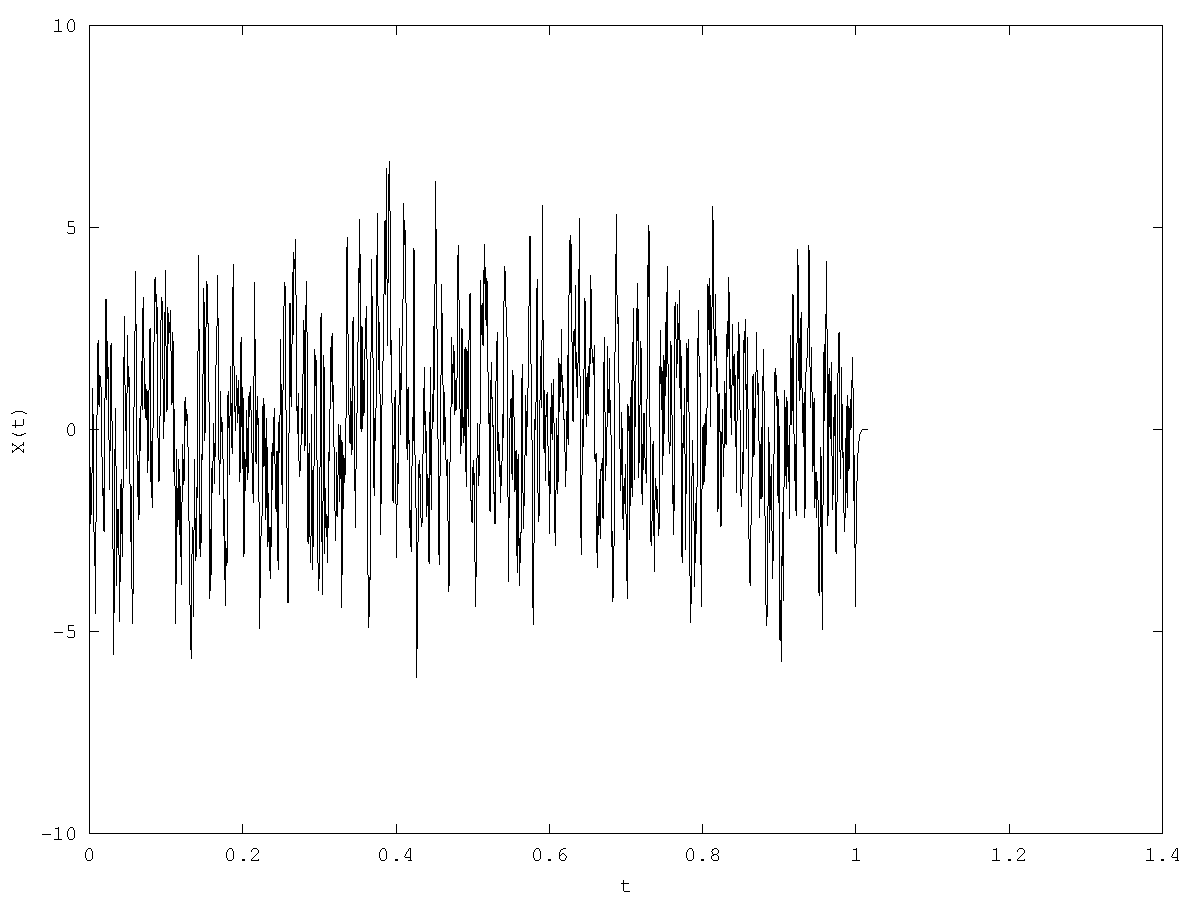
\includegraphics[scale=0.5]{fig1.pdf}
    \end{center}
    \caption{Sýni úr inntaksmerki $X(t)$.}
    \label{fig:X}
\end{figure}
\begin{figure}[htbp]
    \begin{center}
        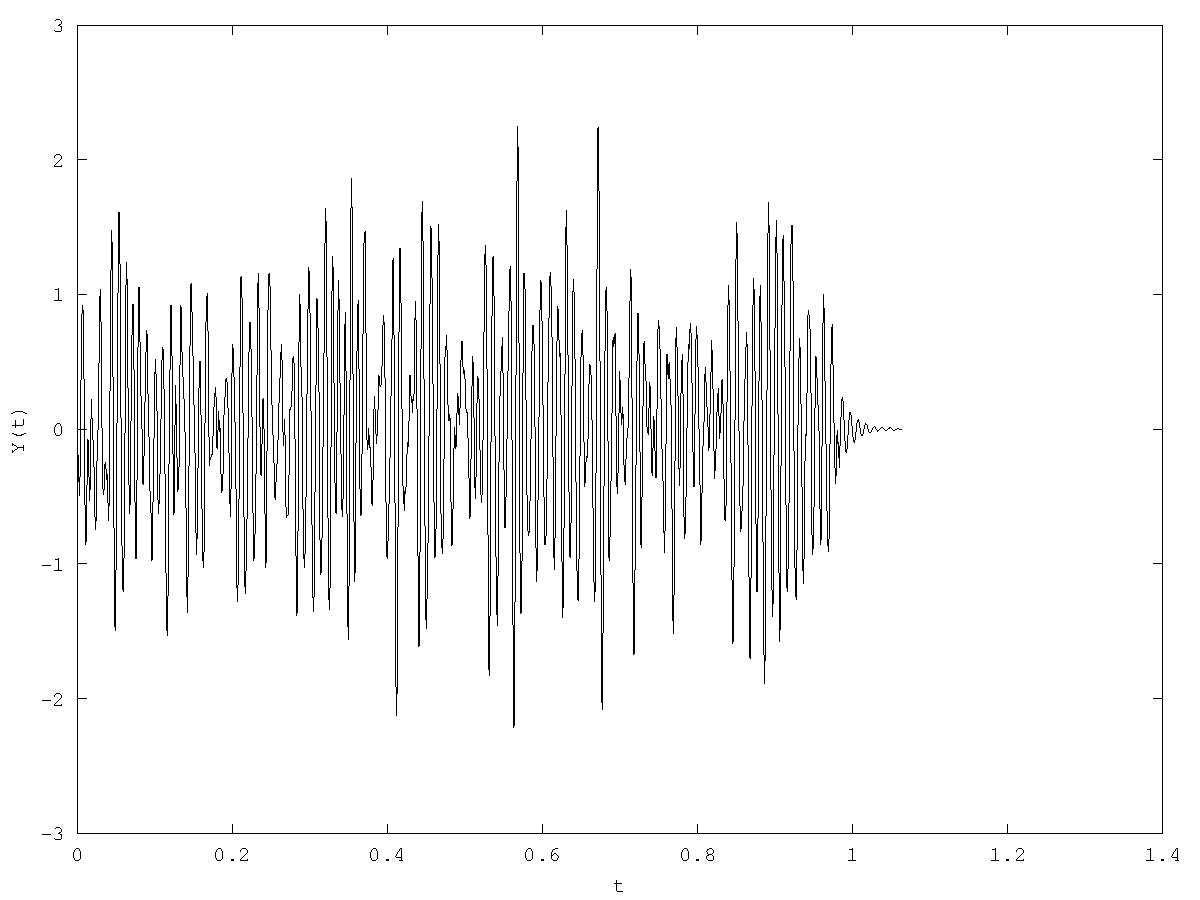
\includegraphics[scale=0.5]{fig2.pdf}
    \end{center}
    \caption{Sýni úr úttakksmerki $Y(t)$.}
    \label{fig:Y}
\end{figure}
\begin{figure}[htbp]
    \begin{center}
        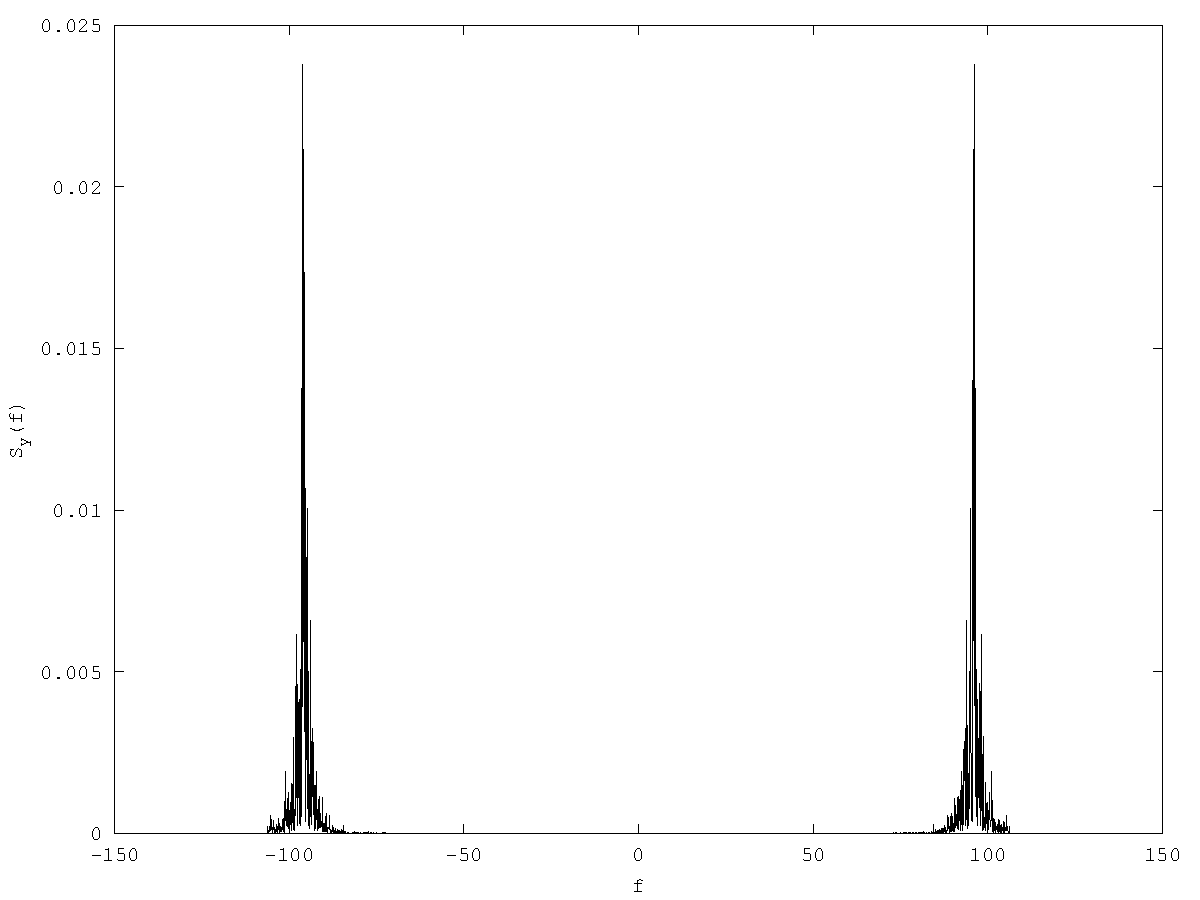
\includegraphics[scale=0.5]{fig3.pdf}
    \end{center}
    \caption{Rófþéttleiki með spect\_est\_pg}
    \label{fig:pg}
\end{figure}
\begin{figure}[htbp]
    \begin{center}
        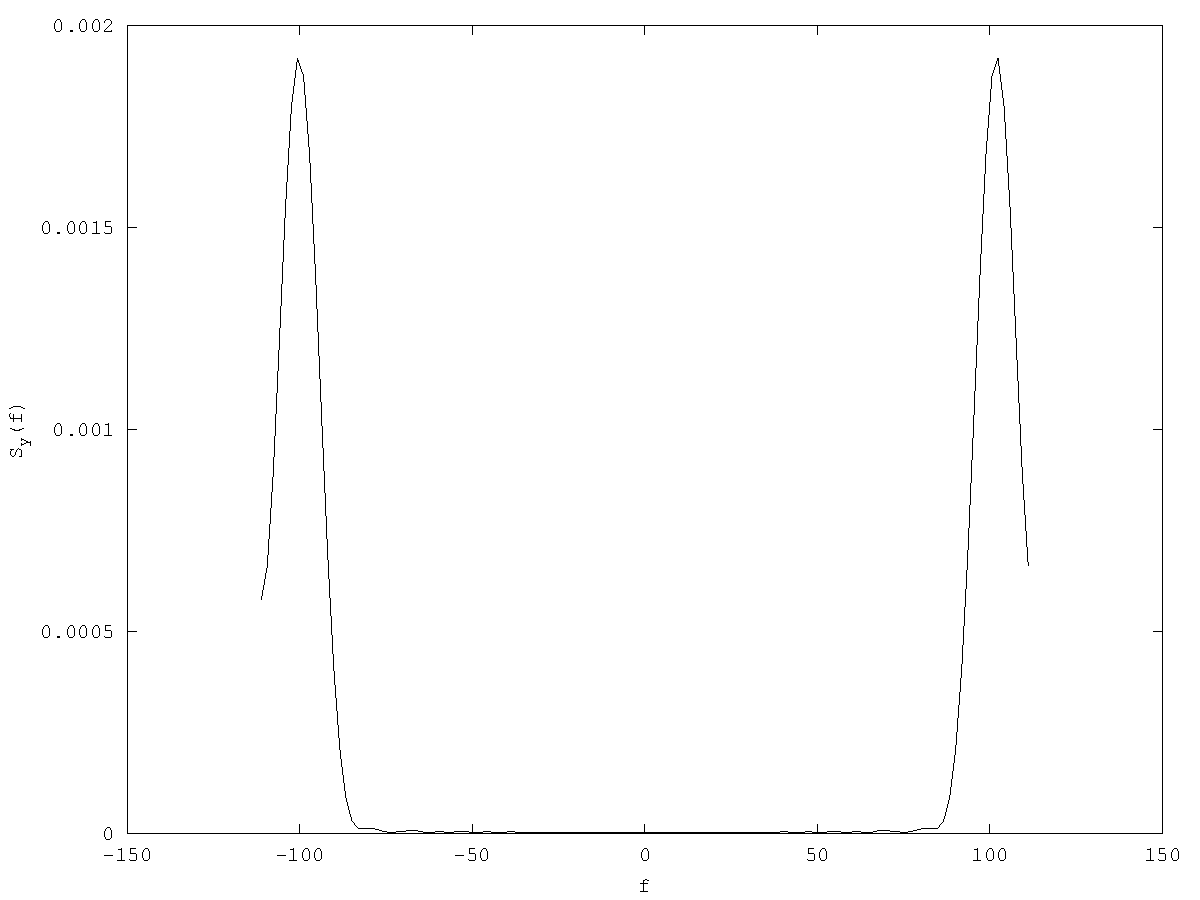
\includegraphics[scale=0.5]{fig4.pdf}
    \end{center}
    \caption{Rófþéttleiki með spect\_est\_ac}
    \label{fig:ac}
\end{figure}
\begin{figure}[htbp]
    \begin{center}
        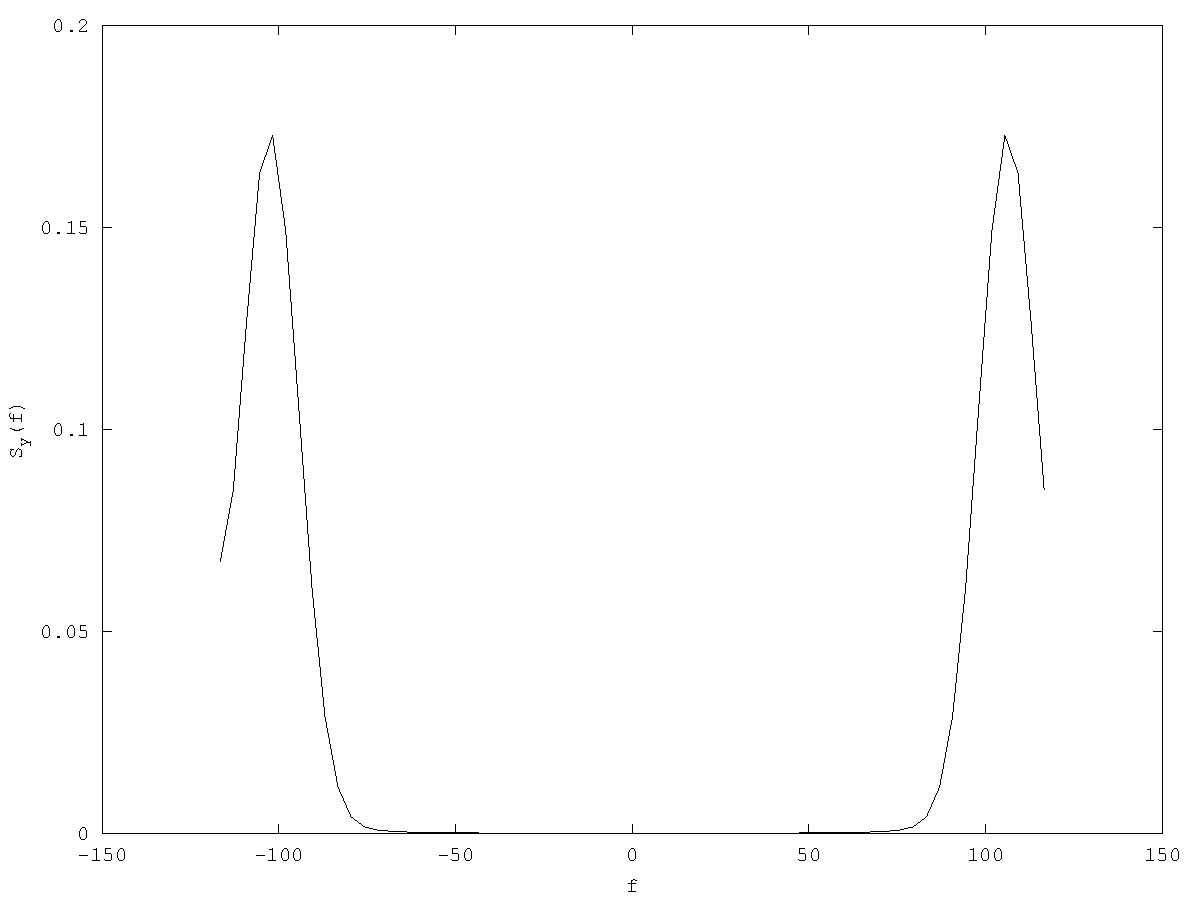
\includegraphics[scale=0.5]{fig5.pdf}
    \end{center}
    \caption{Rófþéttleiki með spect\_est\_x, hamming glugga og nákvæmni í toppgildi.}
    \label{fig:hamming}
\end{figure}
\begin{figure}[htbp]
    \begin{center}
        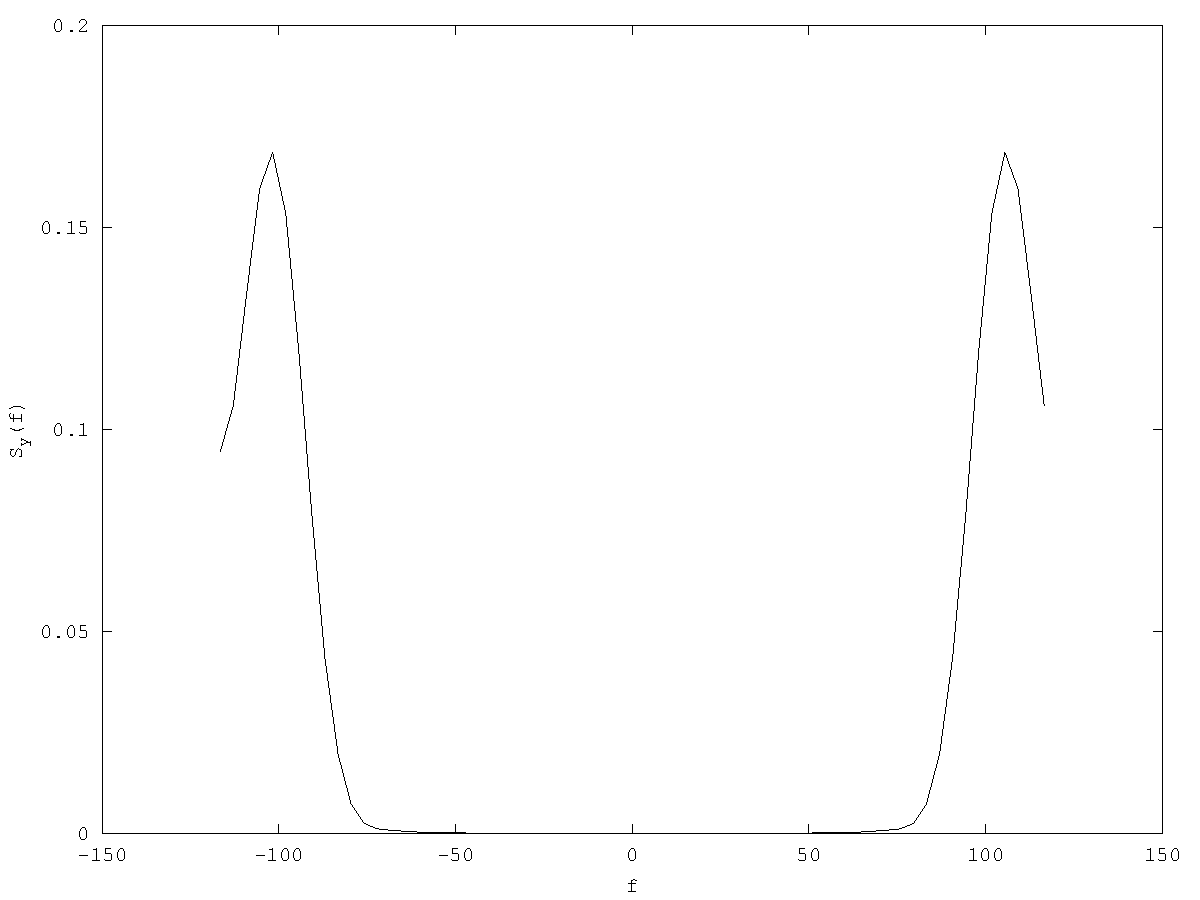
\includegraphics[scale=0.5]{fig6.pdf}
    \end{center}
    \caption{Rófþéttleiki með spect\_est\_x, hamming glugga og nákvæmni í toppgildi.}
    \label{fig:hanning}
\end{figure}
\begin{figure}[htbp]
    \begin{center}
        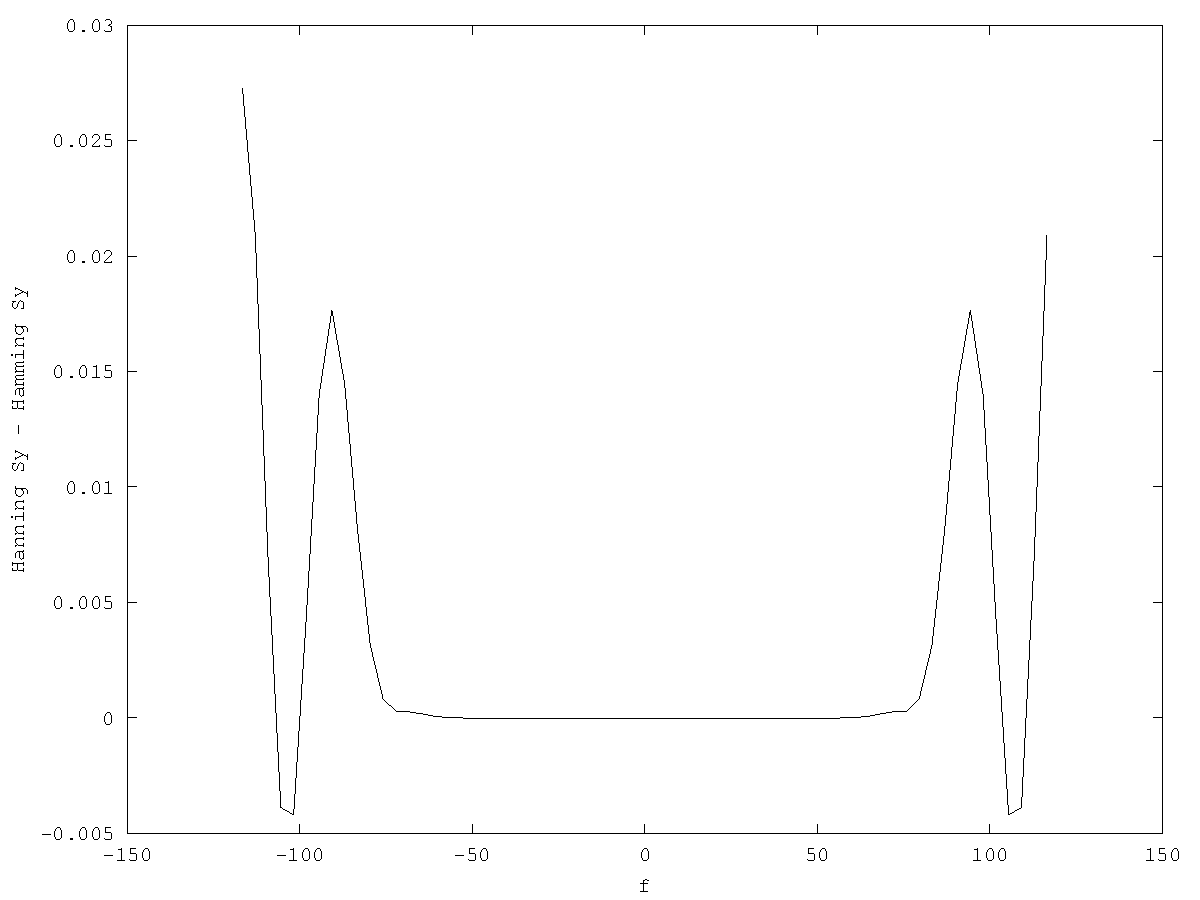
\includegraphics[scale=0.5]{fig7.pdf}
    \end{center}
    \caption{Hamming fundinn rófþéttleiki dreginn frá hanning fundnum rófþéttleika.}
    \label{fig:vs}
\end{figure}
\clearpage
\section{Kóði} \label{se:kodi}
LikVerk3.m
\verbatiminput{LikVerk3.m}
spect\_est\_pg.m
\verbatiminput{spect_est_pg.m}

spect\_est\_ac.m
\verbatiminput{spect_est_ac.m}

spect\_est\_x.m
\verbatiminput{spect_est_x.m}
\end{document}


